%%%%%%%%%%%%%%%%%%%%%%%%%%%%%%%%%%%%%%%%%%%%%%
\section{Penguin dating}
%%%%%%%%%%%%%%%%%%%%%%%%%%%%%%%%%%%%%%%%%%%%%%


\begin{frame}{Analysis of penguin morphological data}

Penguin dataset (Ksepka et al 2012) consisting of morphological data of:
\begin{itemize}
\item all extant penguins (19 species)
\item 36 fossil species assigned to stratigraphic intervals
\end{itemize}

\vskip2mm

Models:

\begin{itemize}
\item Lewis MK vs MKv (Lewis 2001)
\item Partitions vs single alignment
\item Rate variation across sites and across partitions
\item Tree prior: FBD and Skyline FBD
\item Different tree model parameterisations
\end{itemize}


\end{frame}


%%%%%%%%%%%%%%%%%%%%%%%%%%%%%%%%%%%%%%%%%%%%%%

\begin{frame}{Parameterisations}

\renewcommand{\arraystretch}{1.2}

lmp:

\color{newblue1} 

\begin{equation*} 
\begin{tabular}{ll} 
\text{birth rate} & $\lambda$  \\ 
\text{death rate} & $\mu$ \\ 
\text{sampling rate} & $\psi$  \\ 
\textcolor{black}{other parameters} & \textcolor{black}{$t_{or}, \rho$} \\
\end{tabular} \end{equation*}

\textcolor{black}{dvs:}

\begin{equation*} 
\begin{tabular}{ll} 
\text{net diversification rate} & $d = \lambda-\mu$  \\ 
\text{turnover rate} & $\turnover = \frac \mu \lambda$ \\ 
\text{\sampleprop} & $\fosp = \frac\psi {\mu + \psi}$  \\ 
\textcolor{black}{other parameters} & \textcolor{black}{$t_{or}, \rho$} \\
\end{tabular} \end{equation*}



\end{frame}

%%%%%%%%%%%%%%%%%%%%%%%%%%%%%%%%%%%%%%%%%%%%%%



\begin{frame}
\begin{figure}
\includegraphics[width=0.7\textwidth]{../../ag_morpho_data/figures/sa.pdf}
\label{saPostPr}
\end{figure}
\small{Probabilities of each fossil to be a sampled ancestor across models.

{\it P} stands for the partitioned model, {\it G} for gamma variation across sites, {\it Mkv} for conditioning on 
variable characters, {\it R} for relaxed clock model, {\it dns} for $d$, $\nu$, and $s$ tree prior parameterisation, {\it lmp} for $
\lambda$, $\mu$, and $\psi$ tree prior parameterisation.} 
\end{frame}

%%%%%%%%%%%%%%%%%%%%%%%%%%%%%%%%%%%%%%%%%%%%%%

\begin{frame}
\begin{figure}
\includegraphics[width=\textwidth]{../../ag_morpho_data/figures/pp.pdf}
\label{postPredictive}
\end{figure}
\small{The posterior and posterior predictive distributions for (left) tree length, $T$, and genealogical $D_F$ statistics and (right) $B_1$ tree imbalance statistic and Colless's tree imbalance index, $I_c$, for model 8. 

The posterior trees are on the unbalanced end of the predictive distribution.}
\end{frame}

%%%%%%%%%%%%%%%%%%%%%%%%%%%%%%%%%%%%%%%%%%%%%%

\begin{frame}
\begin{figure}
\includegraphics[width=\textwidth]{../../ag_morpho_data/figures/tree.pdf}
\label{penguinTree}
\end{figure}
\footnotesize{A maximum sampled ancestor clade credibility tree for the total-evidence analysis. % with mean node ages. 
The numbers in blue show the posterior supports of clades. The filled red and black circles represent sampled 
ancestors. Fossils with positive evidence of being sampled ancestors are shown in red.}

\end{frame}

%%%%%%%%%%%%%%%%%%%%%%%%%%%%%%%%%%%%%%%%%%%%%%

\begin{frame}
\begin{figure}
\begin{center}
\includegraphics[width=0.75\textwidth]{../../ag_morpho_data/figures/BayesFactors.pdf}
\label{fig:BF}
\end{center}
\end{figure}
\small{The evidence fossil sampled ancestors. The samples above the shaded area have positive evidence to be sampled ancestors and below the shaded area have positive evidence to be terminal nodes.}

\end{frame}

%%%%%%%%%%%%%%%%%%%%%%%%%%%%%%%%%%%%%%%%%%%%%%

\begin{frame}
\begin{figure}
\includegraphics[width=0.95\textwidth]{../../ag_morpho_data/figures/extant_tree.pdf}
\label{fig:divDates}
\end{figure}
\small{The posterior summary tree of extant penguins with 95\% HPD intervals and
posterior supports of clades after removing fossils.}
\end{frame}

%%%%%%%%%%%%%%%%%%%%%%%%%%%%%%%%%%%%%%%%%%%%%%

\begin{frame}
\begin{figure}
\begin{center}
\includegraphics[width=0.75\textwidth]{../../ag_morpho_data/figures/root_ages.pdf}
\label{fig:rootAges}
\end{center}
\end{figure}
\small{The age of root of extant penguins across models including total-evidence analysis under relaxed (8+DNA R) and strict (8+DND S) molecular clocks and 
total-evidence analysis with crown fossils only.}
\end{frame}

%%%%%%%%%%%%%%%%%%%%%%%%%%%%%%%%%%%%%%%%%%%%%%

\begin{frame}
\frametitle{Dating the evolutionary history of penguins}
\begin{figure}
\includegraphics[width=\textwidth]{penguinTree.pdf}
\end{figure}
\end{frame}


%%%%%%%%%%%%%%%%%%%%%%%%%%%%%%%%%%%%%%%%%%%%%%

\begin{frame}{But what about those hyper parameter priors?}
\begin{figure}
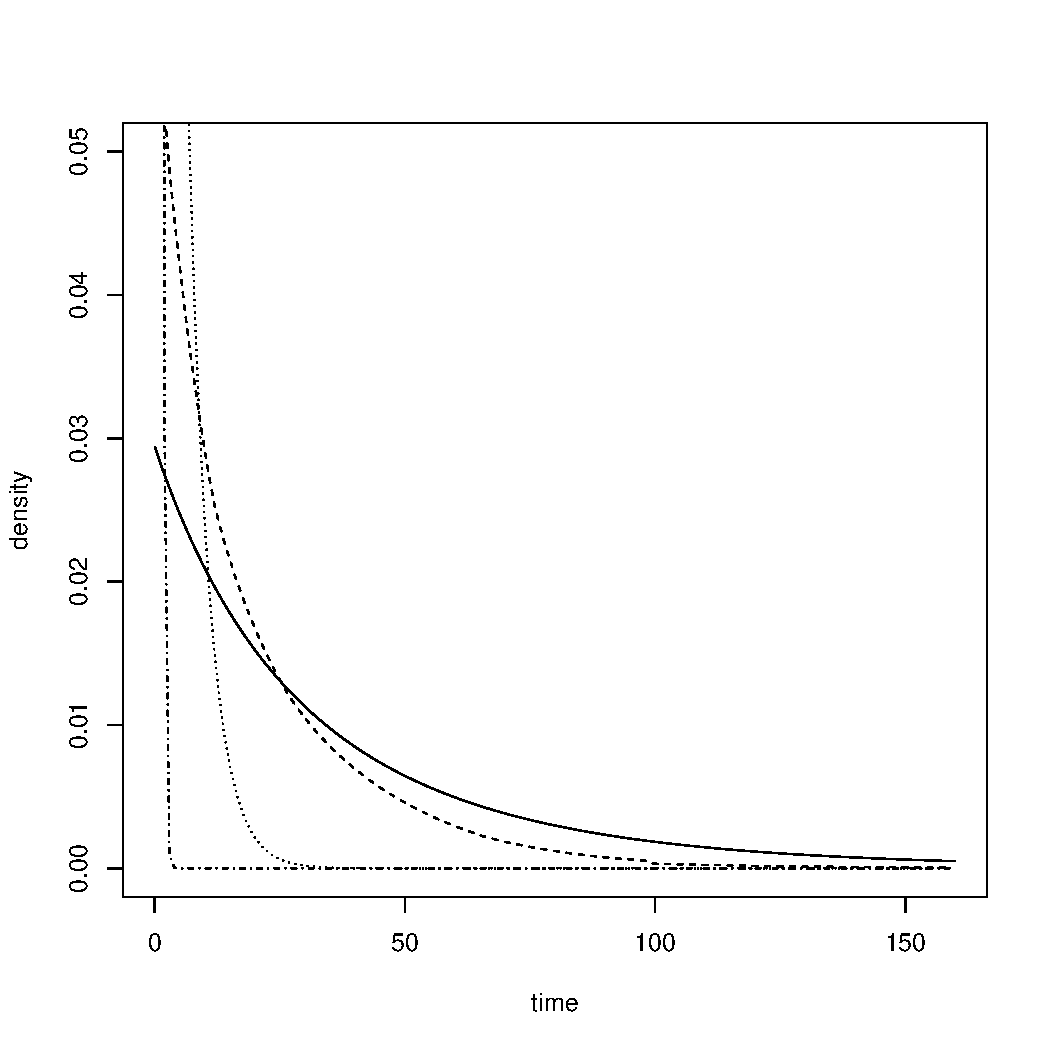
\includegraphics[width=0.6\textwidth]{../priors.pdf}
\label{Fig:Prior}
\end{figure}

\small{Prior density for sampling times under fossilized birth-death process. Dot-dashed line uses priors from \textcite{gavryushkina2015bayesian}. 
Solid line is new prior with implicit assumptions on $T$ and $s$, dashed line results from only assuming implicit prior on $T$,  dotted line results from only assuming implicit prior on $s$.}
\end{frame}

